\subsubsection{13.01.15}
\begin{enumerate}
	
	\item Время начала и окончания собрания: 16:00 - 20:00.
	
	\item Цели собрания: 
	\begin{enumerate}
		
		\item Реализовать синхронное с опрокидыванием ковша раскрытие направляющей для шаров.
		
	\end{enumerate}

	\item Проделанная работа:
	\begin{enumerate}
		
		\item Желоб и направляющая для шаров были доработаны: Место крепления желоба к рейкам было усилено, направляющая подрезана таким образом, чтобы она в сложенном состоянии входила в допустимые размеры, была проведена система синхронного открытия направляющей и ковша.
		\begin{figure}[H]
			\begin{minipage}[h]{0.26\linewidth}
				\center{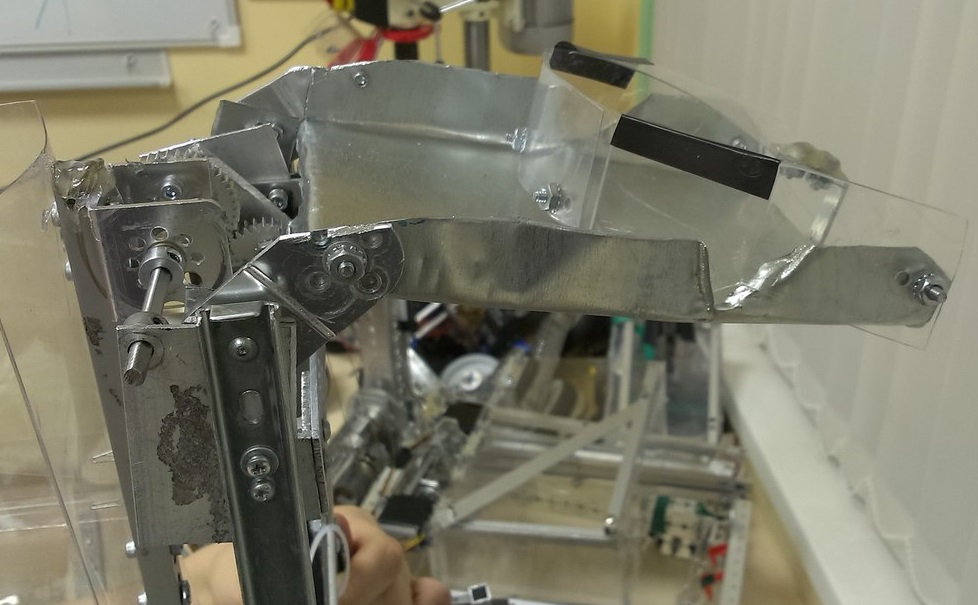
\includegraphics[scale=0.18]{days/13.01.15/images/01}}  
			\end{minipage}
			\hfill
			\begin{minipage}[h]{0.24\linewidth}
				\center{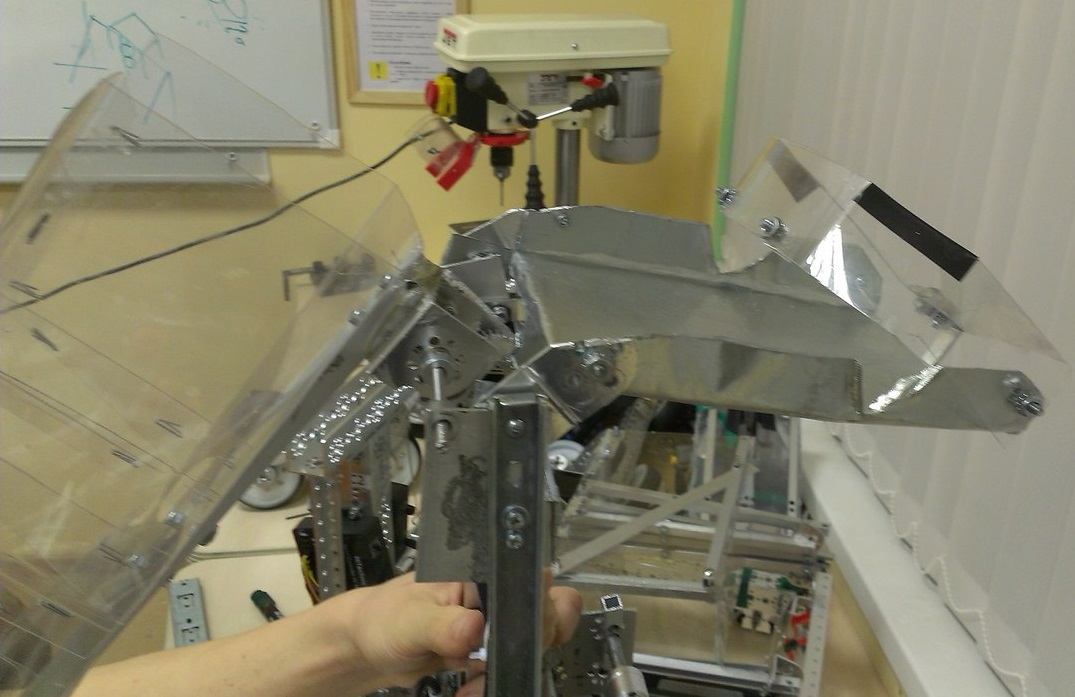
\includegraphics[scale=0.15]{days/13.01.15/images/02}}
			\end{minipage}
			\hfill
			\begin{minipage}[h]{0.24\linewidth}
				\center{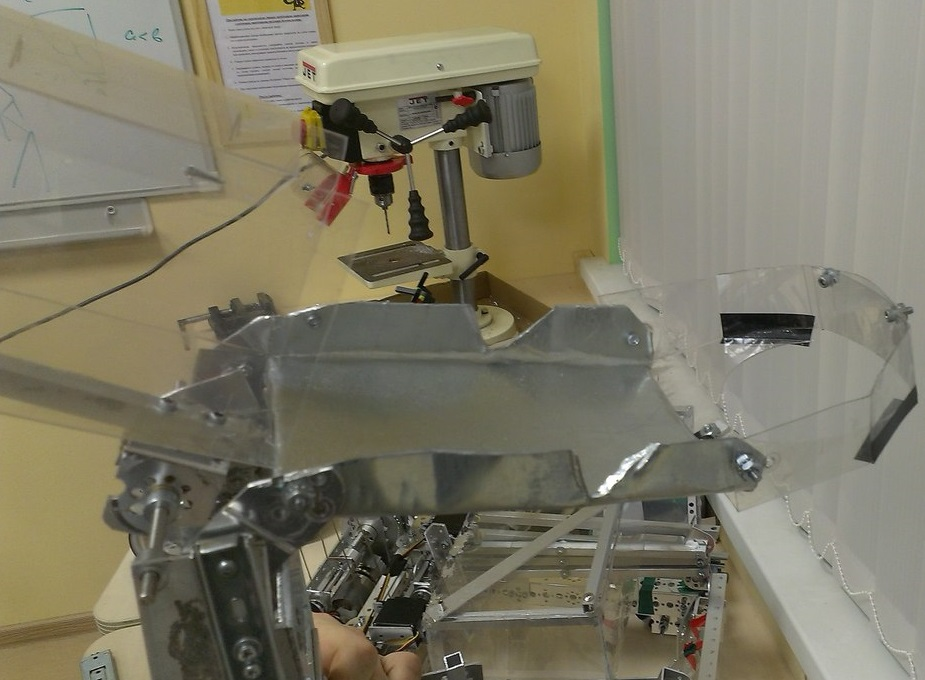
\includegraphics[scale=0.16]{days/13.01.15/images/03}} 
			\end{minipage}
			\caption{Процесс раскрытия направляющей}
		\end{figure}

	\end{enumerate}
	
	\item Итоги собрания:
	\begin{enumerate}
		
		\item Модуль ковша полностью готов и работоспособен.
		
	\end{enumerate}
	
	\item Задачи для последующих собраний:
	\begin{enumerate}
		
		\item Испытать модуль ковша в процессе тренировок.
			
	\end{enumerate}
\end{enumerate}
\fillpage
